
% \section{Primer ap\'endice Comportamientos}
% Mostrar como est\'a implementada la arquitectura como software,
% 
% \section{Segundo ap\'endice Comportamientos}
% que habr\'ia que hacer para agregar un comportamiento nuevo, modificar
% uno existente.
% 
% \section{Tercer ap\'endice Comportamientos}
% Que hay que hacer para agregar un sensor o actuador nuevo.
% 
% \section{Cuarto ap\'endice Comportamientos}
% Que hay que hacer en caso que se modifique el protocolo.
% 
% \section{Quinto ap\'endice Comportamientos}
% Como es la interfaz con vision y porque se hizo de esa forma.

\section[Implementaci\'on del protocolo en PC]{Implementaci\'on del protocolo de comunicaci\'on del lado de la PC}
La implementaci\'on del protocolo en la PC la hicimos en C++, al igual que
el controlador y el m\'odulo de reconocimiento de basuras. Para la misma
implementamos los paquetes descriptos en el protocolo y un servidor de
env\'io y recepci\'on de los mismos a trav\'es del puerto serial. Tambi\'en
implementamos lo que llamamos handlers, quienes son los responsables de
convertir los comandos de la api del robot en paquetes y enviarlos al
servidor, as\'i como tambi\'en de recibir los paquetes de respuesta que
le incumben y proveerlos a la api de una forma que \'esta los entienda.
Mostramos el diagrama de \'esta relaci\'on en la figura
\ref{fig:diag_server_handler_packet}.
\\\indent
Como mencionamos anteriormente, hay un servidor que denominamos packet
server encargado del env\'io y recepci\'on de paquetes. El mismo provee
dos m\'etodos para realizar estas funciones:
\begin{itemize}
	\item{sendPacket:} Su funci\'on es recibir un paquete y encolarlo para
		que el servidor lo env\'ie. Como el servidor es un thread diferente
		al de la api, no se interrumpe la recepci\'on o env\'io de paquetes.
	\item{registerHandler:} Registra un handler para un paquete enviado desde
		una placa con grupo $groupid$ e id de placa $boardid$. Cuando llega
		un paquete de dicha placa, el servidor invoca el m\'etodo
		handlePacket() del handler registrado.
\end{itemize}
La idea del m\'etodo handlePacket es que se limite s\'olo a guardar los
nuevos valores recibidos, ya que durante la invocaci\'on del mismo el
server no recibe ni env\'ia paquetes.
La clase packet provee funciones de utilidad para cualquier tipo de
paquete, tales como c\'alculo y verificaci\'on de CRC, seteo y obtenci\'on
de valores de los campos del paquete, entre otras.
\begin{figure}[h]
	\centering
	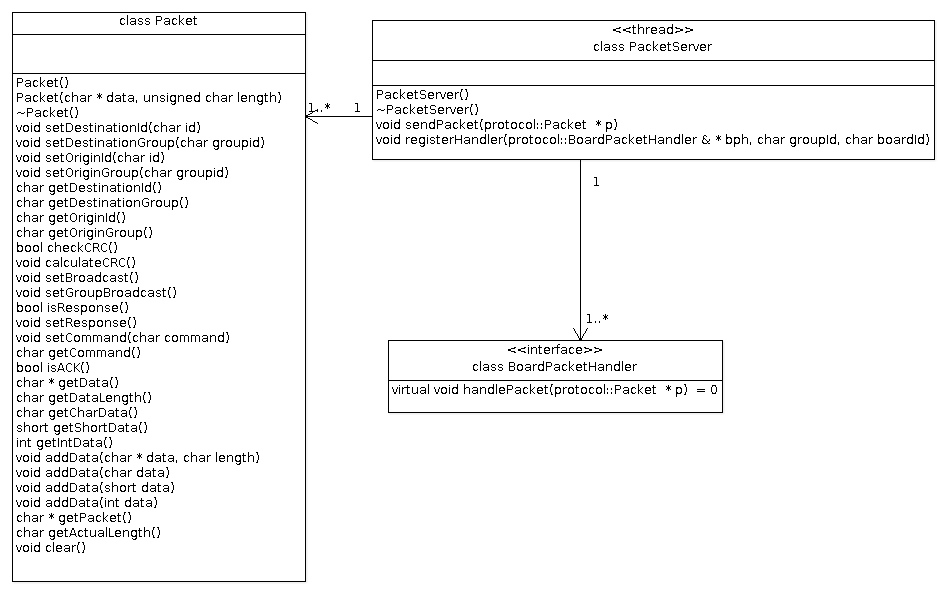
\includegraphics[scale=0.483]{comportamientos/figures/cs4.png}
	\caption[Diagrama de clases: Servidor de paquetes e interface]
			{Diagrama de clases. Estructura general del servidor de paquetes
			e interface para los handlers.}
	\label{fig:diag_server_handler_packet}
\end{figure}
Como indicamos en la figura \ref{packet_group_board}

\begin{figure}[h]
	\centering
	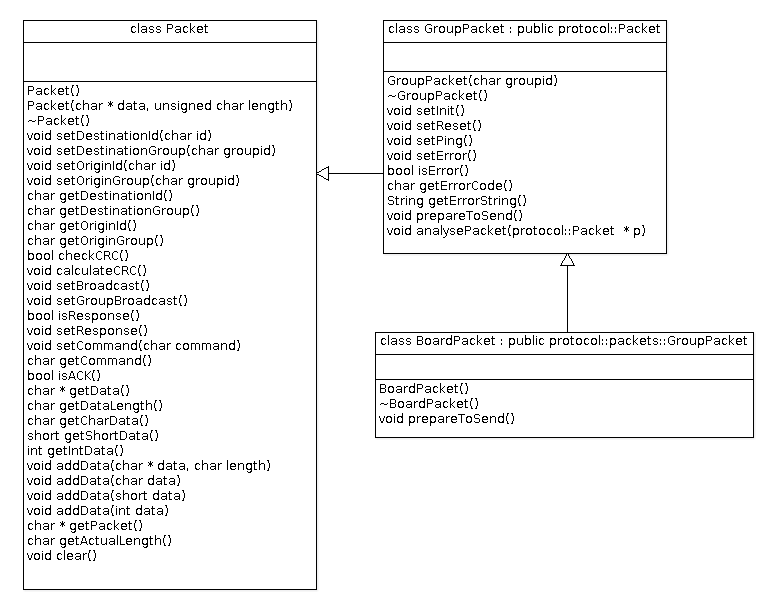
\includegraphics[scale=0.5]{comportamientos/figures/cs1.png}
	\caption[[Diagrama de clases: Estructura general]{Diagrama de clases. Estructura general de los paquetes.}
	\label{fig:packet_group_board}
\end{figure}

\begin{figure}[h]
	\centering
	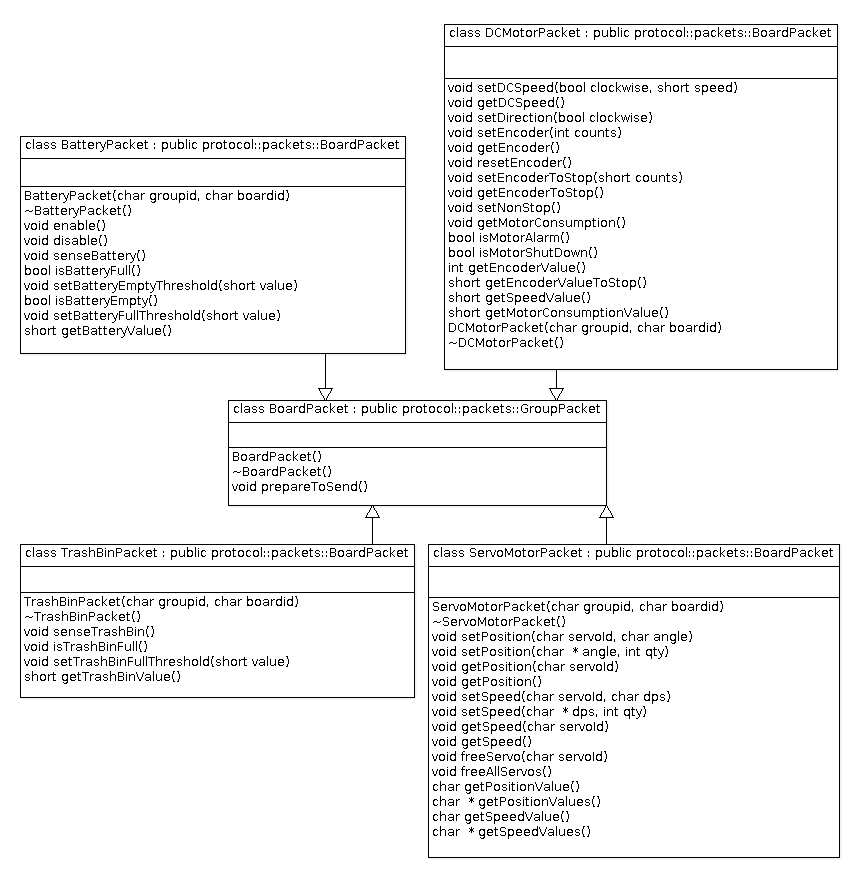
\includegraphics[scale=0.52]{comportamientos/figures/cs2.png}
	\caption[Diagrama de clases: Estructura paquetes 1]{Diagrama de clases. Estructura de los paquetes de motor, recipiente de basura, servos y bater\'ia.}
	\label{fig:diagclases}
\end{figure}

\begin{figure}[h]
	\centering
	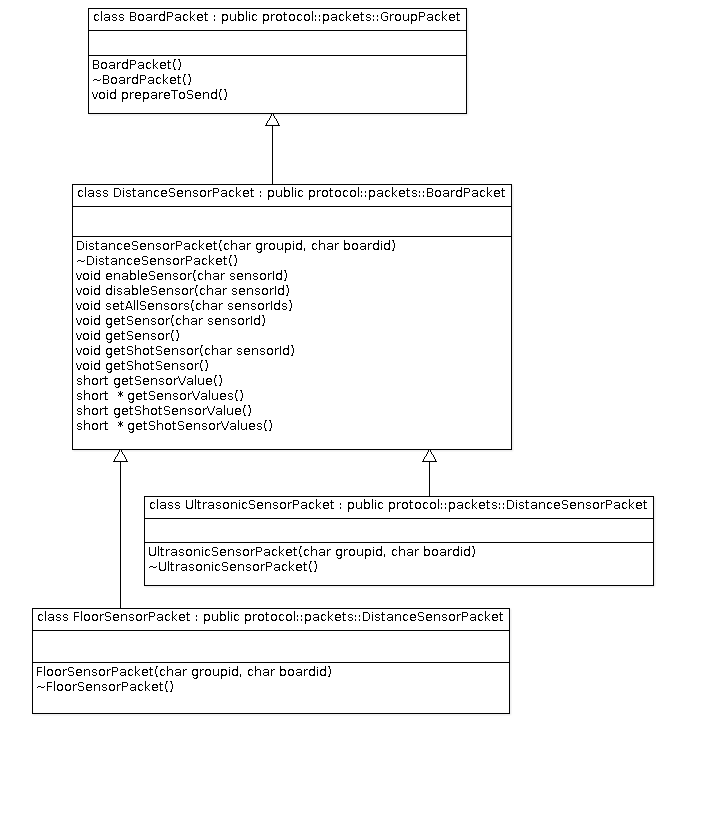
\includegraphics[scale=0.52]{comportamientos/figures/cs3.png}
	\caption[Diagrama de clases: Estructura paquetes 2]{Diagrama de clases. Estructura general de los paquetes para sensores de distancia.}
	\label{fig:diagclases}
\end{figure}

\begin{figure}[h]
	\centering
	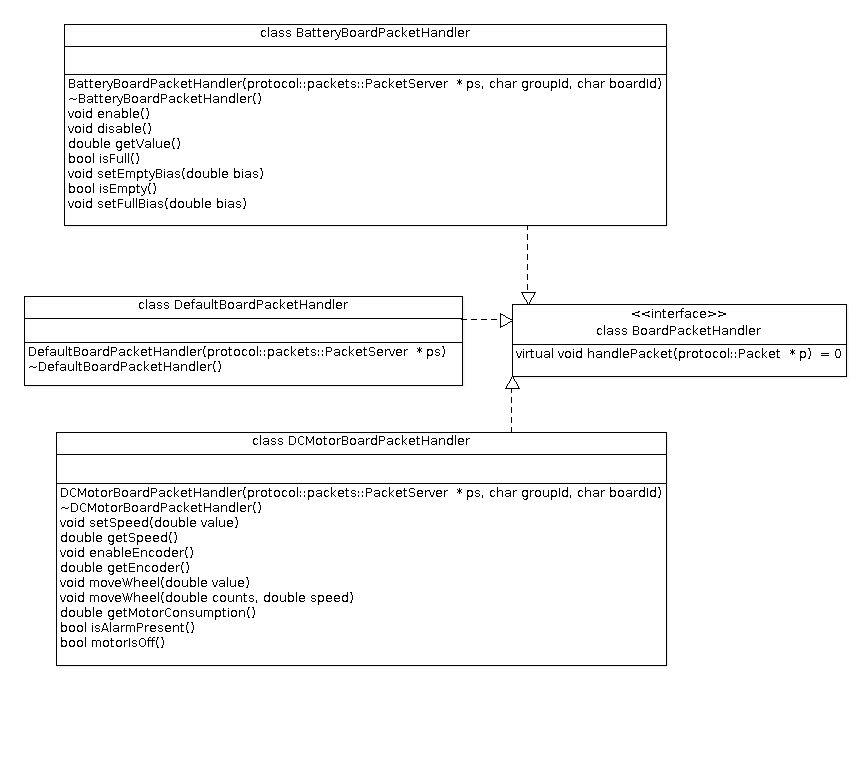
\includegraphics[scale=0.5]{comportamientos/figures/cs5.png}
	\caption[Diagrama de clases: Handlers 1]{Diagrama de clases. Handlers de paquetes default y para las placas de motor y 
	bater\'ia.}
	\label{fig:diagclases}
\end{figure}

\begin{figure}[h]
	\centering
	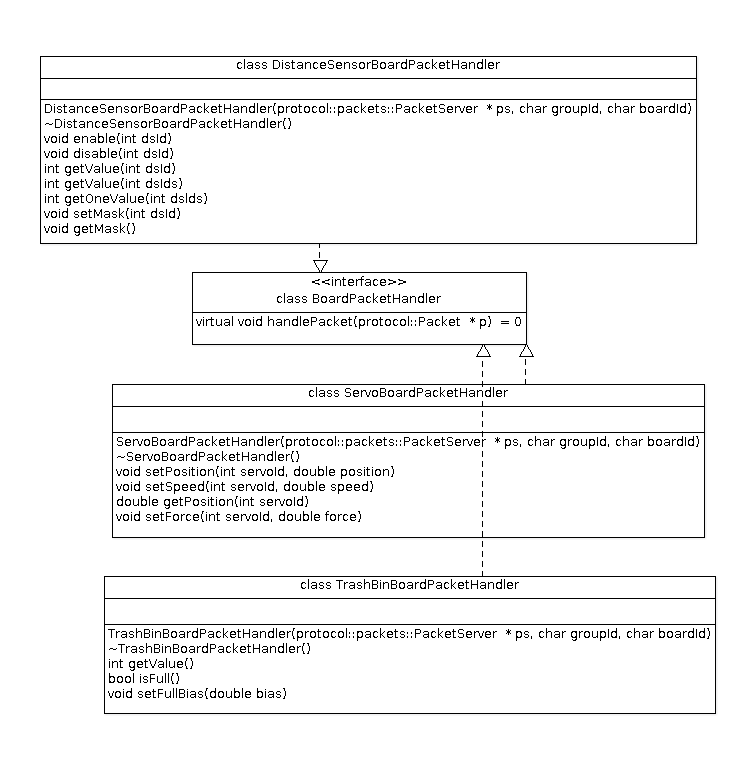
\includegraphics[scale=0.52]{comportamientos/figures/cs6.png}
	\caption[Diagrama de clases: Handlers 2]{Diagrama de clases. Handlers de paquetes para las placas de sensores de 
	distancia, servos y recipiente de residuos.}
	\label{fig:diagclases}
\end{figure}
